
%% bare_conf_compsoc.tex
%% V1.4b
%% 2015/08/26
%% by Michael Shell
%% See:
%% http://www.michaelshell.org/
%% for current contact information.
%%
%% This is a skeleton file demonstrating the use of IEEEtran.cls
%% (requires IEEEtran.cls version 1.8b or later) with an IEEE Computer
%% Society conference paper.
%%
%% Support sites:
%% http://www.michaelshell.org/tex/ieeetran/
%% http://www.ctan.org/pkg/ieeetran
%% and
%% http://www.ieee.org/

%%*************************************************************************
%% Legal Notice:
%% This code is offered as-is without any warranty either expressed or
%% implied; without even the implied warranty of MERCHANTABILITY or
%% FITNESS FOR A PARTICULAR PURPOSE! 
%% User assumes all risk.
%% In no event shall the IEEE or any contributor to this code be liable for
%% any damages or losses, including, but not limited to, incidental,
%% consequential, or any other damages, resulting from the use or misuse
%% of any information contained here.
%%
%% All comments are the opinions of their respective authors and are not
%% necessarily endorsed by the IEEE.
%%
%% This work is distributed under the LaTeX Project Public License (LPPL)
%% ( http://www.latex-project.org/ ) version 1.3, and may be freely used,
%% distributed and modified. A copy of the LPPL, version 1.3, is included
%% in the base LaTeX documentation of all distributions of LaTeX released
%% 2003/12/01 or later.
%% Retain all contribution notices and credits.
%% ** Modified files should be clearly indicated as such, including  **
%% ** renaming them and changing author support contact information. **
%%*************************************************************************


% *** Authors should verify (and, if needed, correct) their LaTeX system  ***
% *** with the testflow diagnostic prior to trusting their LaTeX platform ***
% *** with production work. The IEEE's font choices and paper sizes can   ***
% *** trigger bugs that do not appear when using other class files.       ***                          ***
% The testflow support page is at:
% http://www.michaelshell.org/tex/testflow/



\documentclass[conference,compsoc]{IEEEtran}
% Some/most Computer Society conferences require the compsoc mode option,
% but others may want the standard conference format.
%
% If IEEEtran.cls has not been installed into the LaTeX system files,
% manually specify the path to it like:
% \documentclass[conference,compsoc]{../sty/IEEEtran}





% Some very useful LaTeX packages include:
% (uncomment the ones you want to load)


% *** MISC UTILITY PACKAGES ***
%
%\usepackage{ifpdf}
% Heiko Oberdiek's ifpdf.sty is very useful if you need conditional
% compilation based on whether the output is pdf or dvi.
% usage:
% \ifpdf
%   % pdf code
% \else
%   % dvi code
% \fi
% The latest version of ifpdf.sty can be obtained from:
% http://www.ctan.org/pkg/ifpdf
% Also, note that IEEEtran.cls V1.7 and later provides a builtin
% \ifCLASSINFOpdf conditional that works the same way.
% When switching from latex to pdflatex and vice-versa, the compiler may
% have to be run twice to clear warning/error messages.






% *** CITATION PACKAGES ***
%
\ifCLASSOPTIONcompsoc
  % IEEE Computer Society needs nocompress option
  % requires cite.sty v4.0 or later (November 2003)
  \usepackage[nocompress]{cite}
\else
  % normal IEEE
  \usepackage{cite}
\fi
% cite.sty was written by Donald Arseneau
% V1.6 and later of IEEEtran pre-defines the format of the cite.sty package
% \cite{} output to follow that of the IEEE. Loading the cite package will
% result in citation numbers being automatically sorted and properly
% "compressed/ranged". e.g., [1], [9], [2], [7], [5], [6] without using
% cite.sty will become [1], [2], [5]--[7], [9] using cite.sty. cite.sty's
% \cite will automatically add leading space, if needed. Use cite.sty's
% noadjust option (cite.sty V3.8 and later) if you want to turn this off
% such as if a citation ever needs to be enclosed in parenthesis.
% cite.sty is already installed on most LaTeX systems. Be sure and use
% version 5.0 (2009-03-20) and later if using hyperref.sty.
% The latest version can be obtained at:
% http://www.ctan.org/pkg/cite
% The documentation is contained in the cite.sty file itself.
%
% Note that some packages require special options to format as the Computer
% Society requires. In particular, Computer Society  papers do not use
% compressed citation ranges as is done in typical IEEE papers
% (e.g., [1]-[4]). Instead, they list every citation separately in order
% (e.g., [1], [2], [3], [4]). To get the latter we need to load the cite
% package with the nocompress option which is supported by cite.sty v4.0
% and later.





% *** GRAPHICS RELATED PACKAGES ***
%
\ifCLASSINFOpdf
  \usepackage[pdftex]{graphicx}
%   declare the path(s) where your graphic files are
  \graphicspath{{../pdf/}{../jpeg/}}
%   and their extensions so you won't have to specify these with
%   every instance of \includegraphics
  \DeclareGraphicsExtensions{.pdf,.jpeg,.png}
\else
  % or other class option (dvipsone, dvipdf, if not using dvips). graphicx
  % will default to the driver specified in the system graphics.cfg if no
  % driver is specified.
  % \usepackage[dvips]{graphicx}
  % declare the path(s) where your graphic files are
  % \graphicspath{{../eps/}}
  % and their extensions so you won't have to specify these with
  % every instance of \includegraphics
  % \DeclareGraphicsExtensions{.eps}
\fi
% graphicx was written by David Carlisle and Sebastian Rahtz. It is
% required if you want graphics, photos, etc. graphicx.sty is already
% installed on most LaTeX systems. The latest version and documentation
% can be obtained at: 
% http://www.ctan.org/pkg/graphicx
% Another good source of documentation is "Using Imported Graphics in
% LaTeX2e" by Keith Reckdahl which can be found at:
% http://www.ctan.org/pkg/epslatex
%
% latex, and pdflatex in dvi mode, support graphics in encapsulated
% postscript (.eps) format. pdflatex in pdf mode supports graphics
% in .pdf, .jpeg, .png and .mps (metapost) formats. Users should ensure
% that all non-photo figures use a vector format (.eps, .pdf, .mps) and
% not a bitmapped formats (.jpeg, .png). The IEEE frowns on bitmapped formats
% which can result in "jaggedy"/blurry rendering of lines and letters as
% well as large increases in file sizes.
%
% You can find documentation about the pdfTeX application at:
% http://www.tug.org/applications/pdftex





% *** MATH PACKAGES ***
%
%\usepackage{amsmath}
% A popular package from the American Mathematical Society that provides
% many useful and powerful commands for dealing with mathematics.
%
% Note that the amsmath package sets \interdisplaylinepenalty to 10000
% thus preventing page breaks from occurring within multiline equations. Use:
%\interdisplaylinepenalty=2500
% after loading amsmath to restore such page breaks as IEEEtran.cls normally
% does. amsmath.sty is already installed on most LaTeX systems. The latest
% version and documentation can be obtained at:
% http://www.ctan.org/pkg/amsmath





% *** SPECIALIZED LIST PACKAGES ***
%
%\usepackage{algorithmic}
% algorithmic.sty was written by Peter Williams and Rogerio Brito.
% This package provides an algorithmic environment fo describing algorithms.
% You can use the algorithmic environment in-text or within a figure
% environment to provide for a floating algorithm. Do NOT use the algorithm
% floating environment provided by algorithm.sty (by the same authors) or
% algorithm2e.sty (by Christophe Fiorio) as the IEEE does not use dedicated
% algorithm float types and packages that provide these will not provide
% correct IEEE style captions. The latest version and documentation of
% algorithmic.sty can be obtained at:
% http://www.ctan.org/pkg/algorithms
% Also of interest may be the (relatively newer and more customizable)
% algorithmicx.sty package by Szasz Janos:
% http://www.ctan.org/pkg/algorithmicx




% *** ALIGNMENT PACKAGES ***
%
%\usepackage{array}
% Frank Mittelbach's and David Carlisle's array.sty patches and improves
% the standard LaTeX2e array and tabular environments to provide better
% appearance and additional user controls. As the default LaTeX2e table
% generation code is lacking to the point of almost being broken with
% respect to the quality of the end results, all users are strongly
% advised to use an enhanced (at the very least that provided by array.sty)
% set of table tools. array.sty is already installed on most systems. The
% latest version and documentation can be obtained at:
% http://www.ctan.org/pkg/array


% IEEEtran contains the IEEEeqnarray family of commands that can be used to
% generate multiline equations as well as matrices, tables, etc., of high
% quality.




% *** SUBFIGURE PACKAGES ***
%\ifCLASSOPTIONcompsoc
%  \usepackage[caption=false,font=footnotesize,labelfont=sf,textfont=sf]{subfig}
%\else
%  \usepackage[caption=false,font=footnotesize]{subfig}
%\fi
% subfig.sty, written by Steven Douglas Cochran, is the modern replacement
% for subfigure.sty, the latter of which is no longer maintained and is
% incompatible with some LaTeX packages including fixltx2e. However,
% subfig.sty requires and automatically loads Axel Sommerfeldt's caption.sty
% which will override IEEEtran.cls' handling of captions and this will result
% in non-IEEE style figure/table captions. To prevent this problem, be sure
% and invoke subfig.sty's "caption=false" package option (available since
% subfig.sty version 1.3, 2005/06/28) as this is will preserve IEEEtran.cls
% handling of captions.
% Note that the Computer Society format requires a sans serif font rather
% than the serif font used in traditional IEEE formatting and thus the need
% to invoke different subfig.sty package options depending on whether
% compsoc mode has been enabled.
%
% The latest version and documentation of subfig.sty can be obtained at:
% http://www.ctan.org/pkg/subfig




% *** FLOAT PACKAGES ***
%
%\usepackage{fixltx2e}
% fixltx2e, the successor to the earlier fix2col.sty, was written by
% Frank Mittelbach and David Carlisle. This package corrects a few problems
% in the LaTeX2e kernel, the most notable of which is that in current
% LaTeX2e releases, the ordering of single and double column floats is not
% guaranteed to be preserved. Thus, an unpatched LaTeX2e can allow a
% single column figure to be placed prior to an earlier double column
% figure.
% Be aware that LaTeX2e kernels dated 2015 and later have fixltx2e.sty's
% corrections already built into the system in which case a warning will
% be issued if an attempt is made to load fixltx2e.sty as it is no longer
% needed.
% The latest version and documentation can be found at:
% http://www.ctan.org/pkg/fixltx2e


%\usepackage{stfloats}
% stfloats.sty was written by Sigitas Tolusis. This package gives LaTeX2e
% the ability to do double column floats at the bottom of the page as well
% as the top. (e.g., "\begin{figure*}[!b]" is not normally possible in
% LaTeX2e). It also provides a command:
%\fnbelowfloat
% to enable the placement of footnotes below bottom floats (the standard
% LaTeX2e kernel puts them above bottom floats). This is an invasive package
% which rewrites many portions of the LaTeX2e float routines. It may not work
% with other packages that modify the LaTeX2e float routines. The latest
% version and documentation can be obtained at:
% http://www.ctan.org/pkg/stfloats
% Do not use the stfloats baselinefloat ability as the IEEE does not allow
% \baselineskip to stretch. Authors submitting work to the IEEE should note
% that the IEEE rarely uses double column equations and that authors should try
% to avoid such use. Do not be tempted to use the cuted.sty or midfloat.sty
% packages (also by Sigitas Tolusis) as the IEEE does not format its papers in
% such ways.
% Do not attempt to use stfloats with fixltx2e as they are incompatible.
% Instead, use Morten Hogholm'a dblfloatfix which combines the features
% of both fixltx2e and stfloats:
%
% \usepackage{dblfloatfix}
% The latest version can be found at:
% http://www.ctan.org/pkg/dblfloatfix




% *** PDF, URL AND HYPERLINK PACKAGES ***
%
\usepackage{url}
% url.sty was written by Donald Arseneau. It provides better support for
% handling and breaking URLs. url.sty is already installed on most LaTeX
% systems. The latest version and documentation can be obtained at:
% http://www.ctan.org/pkg/url
% Basically, \url{my_url_here}.




% *** Do not adjust lengths that control margins, column widths, etc. ***
% *** Do not use packages that alter fonts (such as pslatex).         ***
% There should be no need to do such things with IEEEtran.cls V1.6 and later.
% (Unless specifically asked to do so by the journal or conference you plan
% to submit to, of course. )


% correct bad hyphenation here
\hyphenation{op-tical net-works semi-conduc-tor}


\begin{document}
%
% paper title
% Titles are generally capitalized except for words such as a, an, and, as,
% at, but, by, for, in, nor, of, on, or, the, to and up, which are usually
% not capitalized unless they are the first or last word of the title.
% Linebreaks \\ can be used within to get better formatting as desired.
% Do not put math or special symbols in the title.
\title{A Web Serverless Architecture for Buildings Modeling}


% author names and affiliations
% use a multiple column layout for up to three different
% affiliations

% \author{\IEEEauthorblockN{Michael Shell}
% \IEEEauthorblockA{School of Electrical and\\Computer Engineering\\
% Georgia Institute of Technology\\
% Atlanta, Georgia 30332--0250\\
% Email: http://www.michaelshell.org/contact.html}
% \and
% \IEEEauthorblockN{Homer Simpson}
% \IEEEauthorblockA{Twentieth Century Fox\\
% Springfield, USA\\
% Email: homer@thesimpsons.com}
% \and
% \IEEEauthorblockN{James Kirk\\ and Montgomery Scott}
% \IEEEauthorblockA{Starfleet Academy\\
% San Francisco, California 96678-2391\\
% Telephone: (800) 555--1212\\
% Fax: (888) 555--1212}}

% conference papers do not typically use \thanks and this command
% is locked out in conference mode. If really needed, such as for
% the acknowledgment of grants, issue a \IEEEoverridecommandlockouts
% after \documentclass

% for over three affiliations, or if they all won't fit within the width
% of the page (and note that there is less available width in this regard for
% compsoc conferences compared to traditional conferences), use this
% alternative format:
% 

\author{\IEEEauthorblockN{Enrico Marino\IEEEauthorrefmark{1},
Danilo Salvati\IEEEauthorrefmark{2},
Federico Spini\IEEEauthorrefmark{1}, 
Christian Vadal\`a\IEEEauthorrefmark{2}}
\IEEEauthorblockA{\IEEEauthorrefmark{1}Department of Engineering, Roma Tre University, Rome, Italy\\
Email:\{marino,spini\}@ing.uniroma3.it}
\IEEEauthorblockA{\IEEEauthorrefmark{2}Department of Mathematics and Physics, Roma Tre University, Rome, Italy\\
Email:\{salvati,vadala\}@ing.uniroma3.it}}

% \author{\IEEEauthorblockN{Michael Shell\IEEEauthorrefmark{1},
% Homer Simpson\IEEEauthorrefmark{2},
% James Kirk\IEEEauthorrefmark{3}, 
% Montgomery Scott\IEEEauthorrefmark{3} and
% Eldon Tyrell\IEEEauthorrefmark{4}}
% \IEEEauthorblockA{\IEEEauthorrefmark{1}School of Electrical and Computer Engineering\\
% Georgia Institute of Technology,
% Atlanta, Georgia 30332--0250\\ Email: see http://www.michaelshell.org/contact.html}
% \IEEEauthorblockA{\IEEEauthorrefmark{2}Twentieth Century Fox, Springfield, USA\\
% Email: homer@thesimpsons.com}
% \IEEEauthorblockA{\IEEEauthorrefmark{3}Starfleet Academy, San Francisco, California 96678-2391\\
% Telephone: (800) 555--1212, Fax: (888) 555--1212}
% \IEEEauthorblockA{\IEEEauthorrefmark{4}Tyrell Inc., 123 Replicant Street, Los Angeles, California 90210--4321}}


% use for special paper notices
%\IEEEspecialpapernotice{(Invited Paper)}




% make the title area
\maketitle

% As a general rule, do not put math, special symbols or citations
% in the abstract
\begin{abstract}
The motivations of relentless migration of software products toward services accessible via Web must be sought in the undeniable benefits in terms of accessibility, usability, maintainability and spreadability granted by the Web medium itself. It is the case of office suites, beforehand thought as resilient desktop applications, nowadays made available as Web applications, often equipped with real-time collaboration features and with no need for the user to explicitly install or upgrade them anymore. Although it could not be easy to envisage a Web-based graphic application due to its inherent complexity, after the recent and significant enrichment of the HTML5 APIs, a few first attempts appeared online in the form of vectorial drawing collaborative editors or VR oriented interior design environments.
This paper introduces an effective Web architecture for buildings modeling that leverages the serverless pattern to dominate the developing complexity. The resulting front-end application, powered by Web Components and based on unidirectional data flow pattern, is extremely customizable and extendible by means the definition of plugins to augment the UI or the application functionalities. As regards the modeling approach, it offers (a) to model the building drawing the 2D plans and to navigate the building in a 3D first person point of view; (b) to collaborate in real-time, allowing to work simultaneously on different layers of the project; (c) to define and use new building elements, that are furnitures or architectural components (such as stairs, roofs, etc.), augmenting a ready to use catalog. This work suggests a path for the next-coming BIM online services, matching the professionals collaboration requirements typical of the BIM approach with the platform which supports them the most: the Web.
\end{abstract}

% no keywords




% For peer review papers, you can put extra information on the cover
% page as needed:
% \ifCLASSOPTIONpeerreview
% \begin{center} \bfseries EDICS Category: 3-BBND \end{center}
% \fi
%
% For peerreview papers, this IEEEtran command inserts a page break and
% creates the second title. It will be ignored for other modes.
\IEEEpeerreviewmaketitle


\section{Introduction}

Scopo di questo lavoro \`e quello di presentare uno strumento di progettazione architettonica basato su web. Dal punto di vista architetturale, \`e stata introdotta una serverless architecture (vedi~\cite{Roberts}). Un'architettura di questo tipo si basa massivamente su servizi di terze parti (typically in the cloud) o su funzioni invocate all'interno di ephemeral containers (may only last for one invocation) per la gestione dello stato e della logica server-side.

Questo strumento si propone di realizzare modelli di edifici attraverso l'introduzione di un'interfaccia semplificata che mira ad evitare complicate interazioni con i modelli tridimensionali cercando invece di rimpiazzarle con interazioni su rappresentazioni bidimensionali simboliche dell'edificio.

La natura web ha permesso di sperimentare API per la collaborazione tra utenti remoti, che possono cos\`i progettare un edificio contemporaneamente su pc diversi.

Molta cura \`e stata poi posta sull'espandibilit\`a del sistema, dando agli sviluppatori un elevato livello di personalizzazione. Ci\`o \`e possibile: (i) Sfruttando \textbf{web components pattern} per aggiungere nuove funzionalità; (ii) introducendo un \textbf{catalogo} personalizzabile, in grado di fornire elementi architetturali specifici del contesto in cui l'applicazione viene utilizzata; (iii) introducendo un gestore dinamico di \textbf{metadati}, in grado di 
attribuire informazioni su ogni componente dell'edificio.

Le sezioni che seguono mostrano nel dettaglio i concetti espressi qui, mostrandone la realizzazione e ponendo l'accento sugli aspetti architetturali. In particolare:\\\\
Nella sezione~\ref{sec:literature} vedremo alcuni lavori correlati per quanto riguarda la modellazione in ambito web osservando pregi e difetti del nostro lavoro.\\\\
Nella sezione~\ref{sec:methodology} studieremo il lavoro vero e proprio, introducendo e commentando le scelte architetturali\\\\
Nella sezione~\ref{sec:results} osserveremo il risultato delle scelte metodologiche effettuate, commentando gli sviluppi futuri del progetto\\\\
\section{Related work}\label{sec:related_work}

In this section we highlight some remarkable experiences aligned with the aim of our project. There are plenty of Desktop applications worth to be mentioned and analyzed, but in the following we deliberately focus on Web based works. 

\textbf{Shapespark}\footnote{https://www.shapespark.com/} offers a web viewer of remarkable quality that allow the user to move inside a synthetic 3D indoor environment. Modeling phase is served in the form of plugins for different Desktop proprietary solutions.

\textbf{Playcanvas}\footnote{https://playcanvas.com/} is a complete and powerful web based game creation platform which offers an integrated physical engine and a whole set of functionalities to support modeling. Although powerful and relatively simple to use, it doesn't focus on buildings modeling.

\textbf{Floorplan}\footnote{http://www.homestyler.com/floorplan/} has been developed by Autodesk specifically for the architectural field, and for indoor renewal projects in particular. It is a 2D modeling tool which offer also a 3D walk-through mode.

Spini et al. \cite{Spini:2016:WIA:2945292.2945309} introduced a Web modeling and baking service for indoor environments. The modeling tools exposes a 3D interaction the user may not be accustomed to, an hitch we tried to outflank by avoiding 3D modeling interaction and let the user only face a ``metaphoric" 2D interface.
\section{Application Experience}\label{sec:application}

The application experience focus on supporting the user in a building modeling task. The exploited modeling approach requires the user to face as much as possible a bidimensional interface which allows her to define the floorplan and to place complex architectural elements (here called \emph{building elements}) on it. Such \emph{building elements} can be found in a pre-filled catalog, and when required can be further configured and customized through a side panel. This modeling approach move part of the complexity toward the developer of the customizable building elements, leaving to the final user the task to place and to configure the employed elements. A rich catalog of elements is thus crucial to answer to the users' modeling requirements.

Once the floorplan has been defined according to the \emph{place-and-configure} approach, the system can automatically generate a 3D model which can be explored externally or in first person view, as shown in Figure~\ref{FIGURA_IN_PRIMA_PERSONA}. Each  \emph{building element} in fact comprises either a \emph{2D generating function} than a \emph{3D generating function}, used to obtain models respectively used in the 2D floorplan definition and in 3D generated model.

The tool also has support for layers the user can exploit to organize her project, for example to group together semantically homogenous elements.

\subsection{Building Elements}\label{ssec:elements}

Along with the aforementioned 2D and 3D generating functions, an elements is fully specified by its univocal name and its properties, used by the user for customization. Each building element inherits from its \emph{prototype} (one and only one). In the prototype are mapped both the inherent characteristics and user interactions needed to add the element to the project and/or configure it.

The catalog comprises then four different types of elements:\\\\
\noindent \emph{Lines}. An element which belongs to this category is drawn selecting a start point and an end point. To move it one can drags one of the end point or can drags the entire line. An example: a \emph{wall}.\\\\
\noindent \emph{Openings}. An opening is an element that is linked to an element of the \emph{line} type, making an hole on it. The user create a new opening by dragging on a chosen line. Examples are \emph{doors} and \emph{windows}.\\\\
\noindent \emph{Areas}. An area is an element which is normally generated by insertion of the boundary vertices. For example a room basement is an area. In this case it is automatically generated from the lines representing walls, thanks to an algorithm which looks for closed cycles. The algorithm is composed by the following phases: (i) search of biconnected component by mean of Hopcroft-Tarjan algorithm~(see \cite{Hopcroft:1973:AEA:362248.362272}); (ii) removal of edges that are not part of a biconnected component; (iii) search of all cycles through an algorithm that do a double check of each edges sorted by angle; (iv) search of maximal cycles correspondent to perimeter edges by an application of Gauss's area formula; (v) removal of maximal cycles.\\\\
\noindent \emph{Object}. An element that is freely inserted into space with a drag and drop interaction is an object. Examples are tables and chairs.\\\

% The internal representation for Line types (e.g. walls) is undirected graph: each node maps coordinates of one tip of the line, each edge represents topological adjacency between vertex. This internal representation helps us to provide a drag and drop interaction for this element type, in fact each drag is performed by means of a relocation od a node that cause, other that the displacement of the requested wall, a displacement of each adjacent wall.


% Areas are automatically generated thanks to an analysis of the wall graph. The algorithm is composed by the following phases: (i) search of biconnected component by mean of Hopcroft-Tarjan algorithm~(see \cite{Hopcroft:1973:AEA:362248.362272}); (ii) removal of edges that are not part of a biconnected component; (iii) search of all cycles through an algorithm that do a double check of each edges sorted by angle; (iv) search of maximal cycles correspondent to perimeter edges by an application of Gauss's area formula; (v) removal of maximal cycles;


\subsection{User Interface}\label{ssec:ui}

\begin{figure}[htb]
\centering
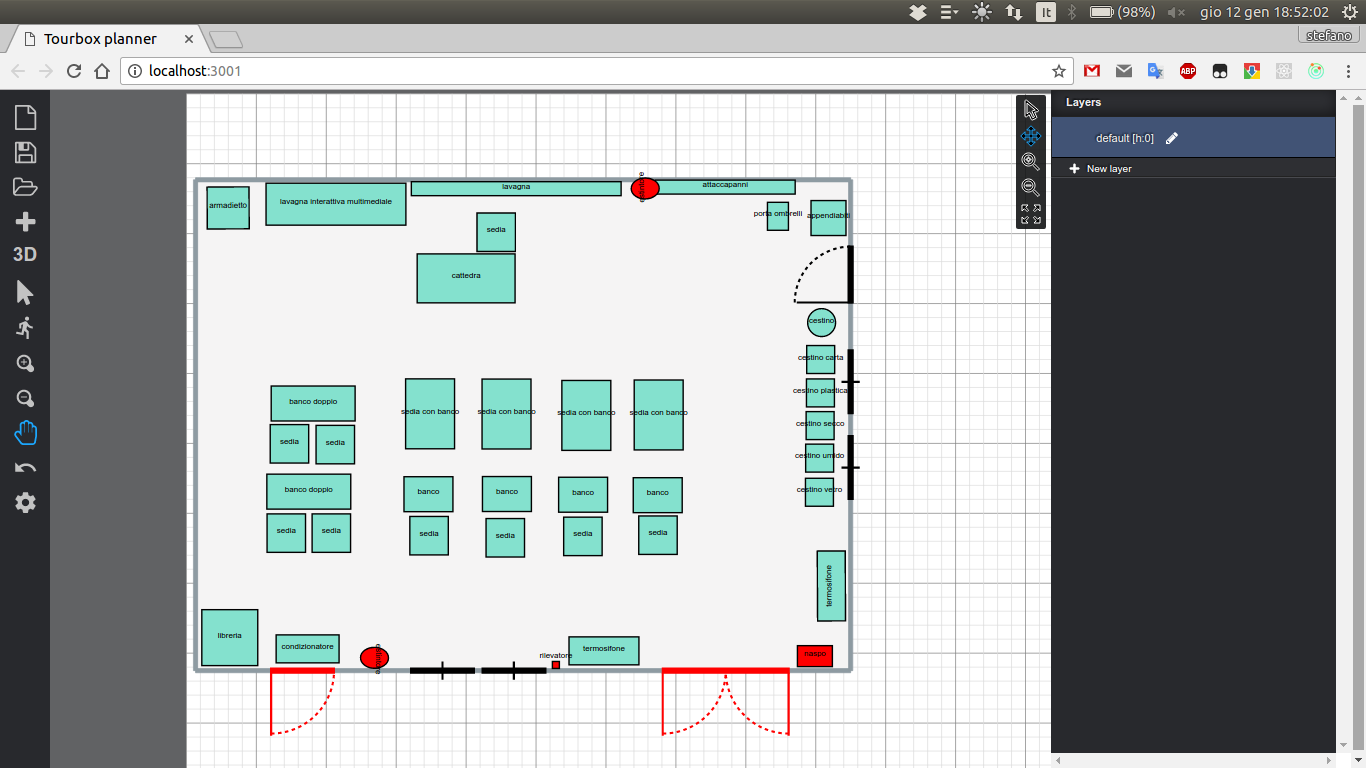
\includegraphics[width=\linewidth]{contents/images/fig2d}
\caption{The user interface}
\label{fig2D}
\end{figure}

Figure~\ref{fig2D} show the application user interface. It consists of the following components (from \textit{left} to \textit{right}):

\textbf{Toolbar:} it contains the button buttons mapping all operations the user can do in that context

\textbf{Content area}: it displays the main content requested by the user. In figure~\ref{fig2D} the content area shows the 2D drawing area.

\textbf{Sidebar:} it contains all elements in the current layer, the layer list and the properties for the selected building element\\

\begin{figure}[htb]
\centering
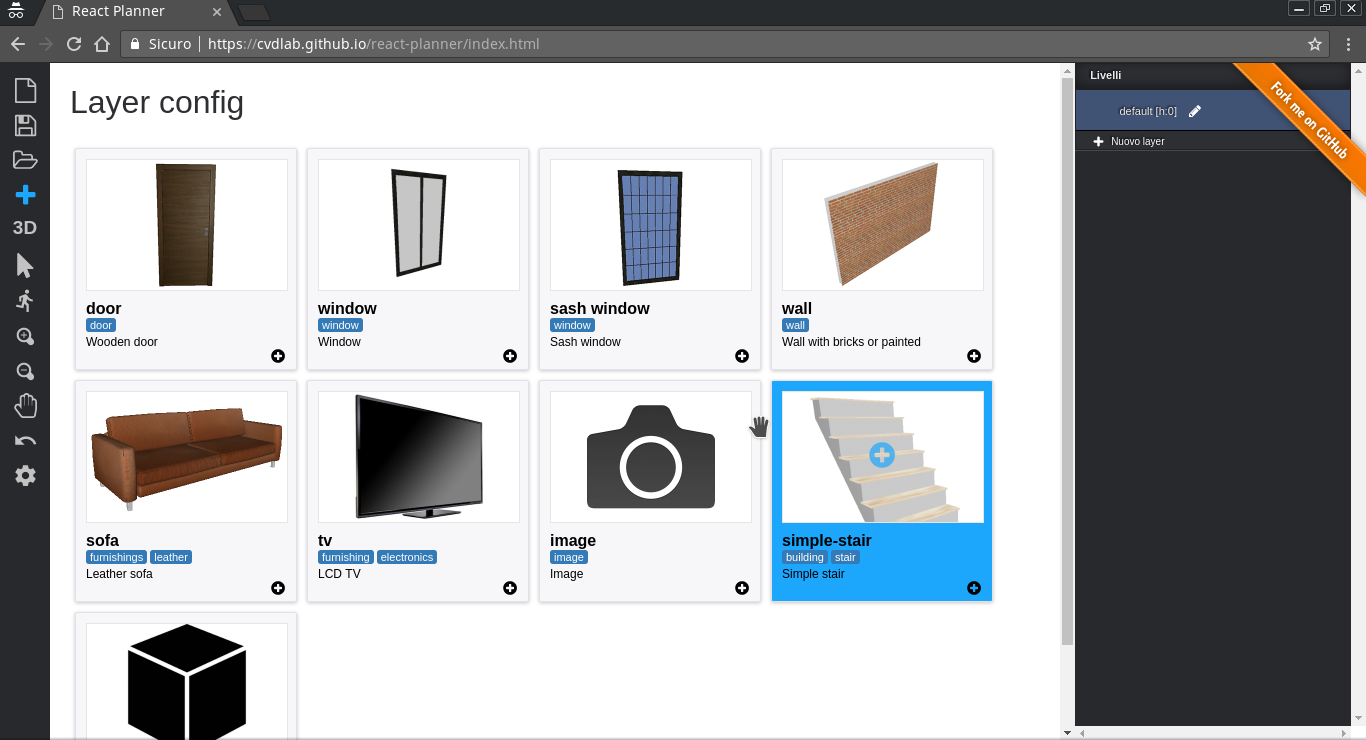
\includegraphics[width=\linewidth]{contents/images/figcatalog}
\caption{The building elements catalog}
\label{figCatalogo}
\end{figure}


Figure~\ref{figCatalogo} shows the building element catalog. When the user select one of the boxes, the application shows the 2D area and starts the interaction for the chosen building element.

\begin{figure}[htb]
\centering
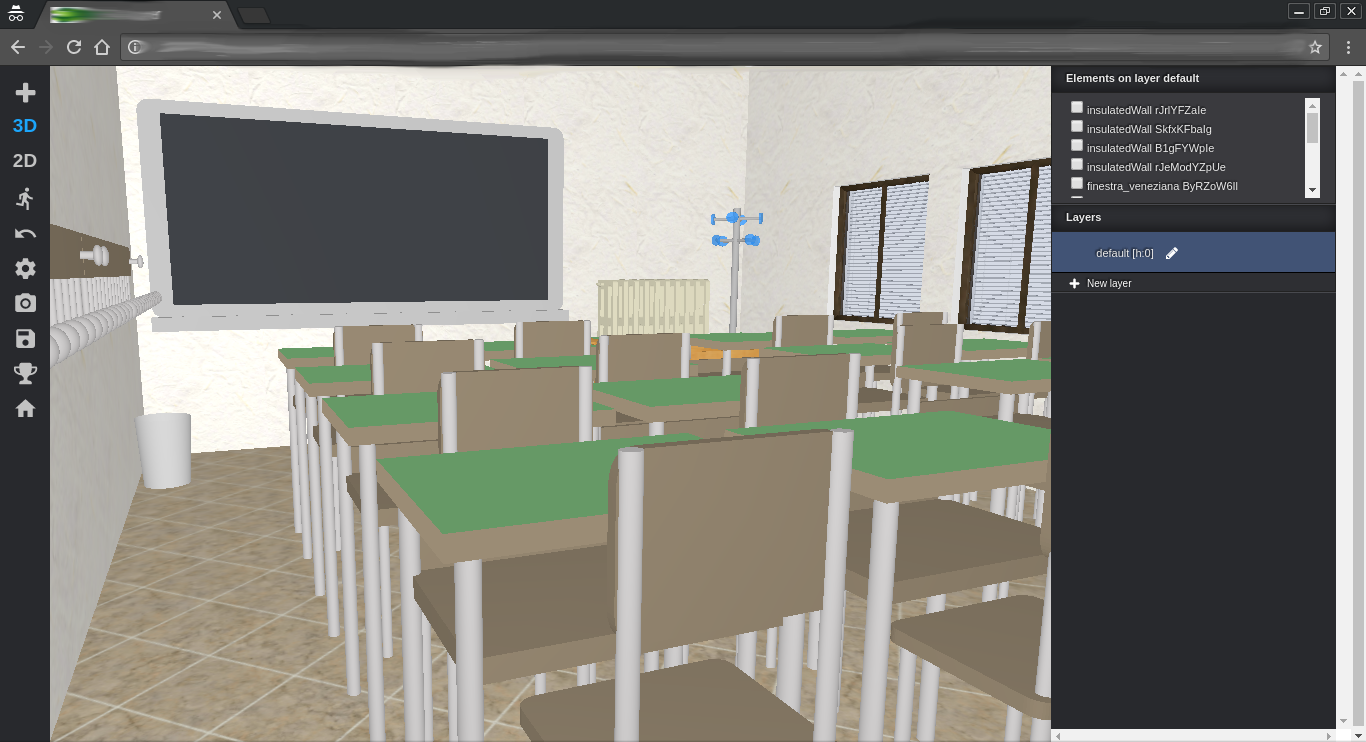
\includegraphics[width=\linewidth]{contents/images/3d-school}
\caption{3D visualization of a school}
\label{fig3D-school}
\end{figure}

\begin{figure}[htb]
\centering
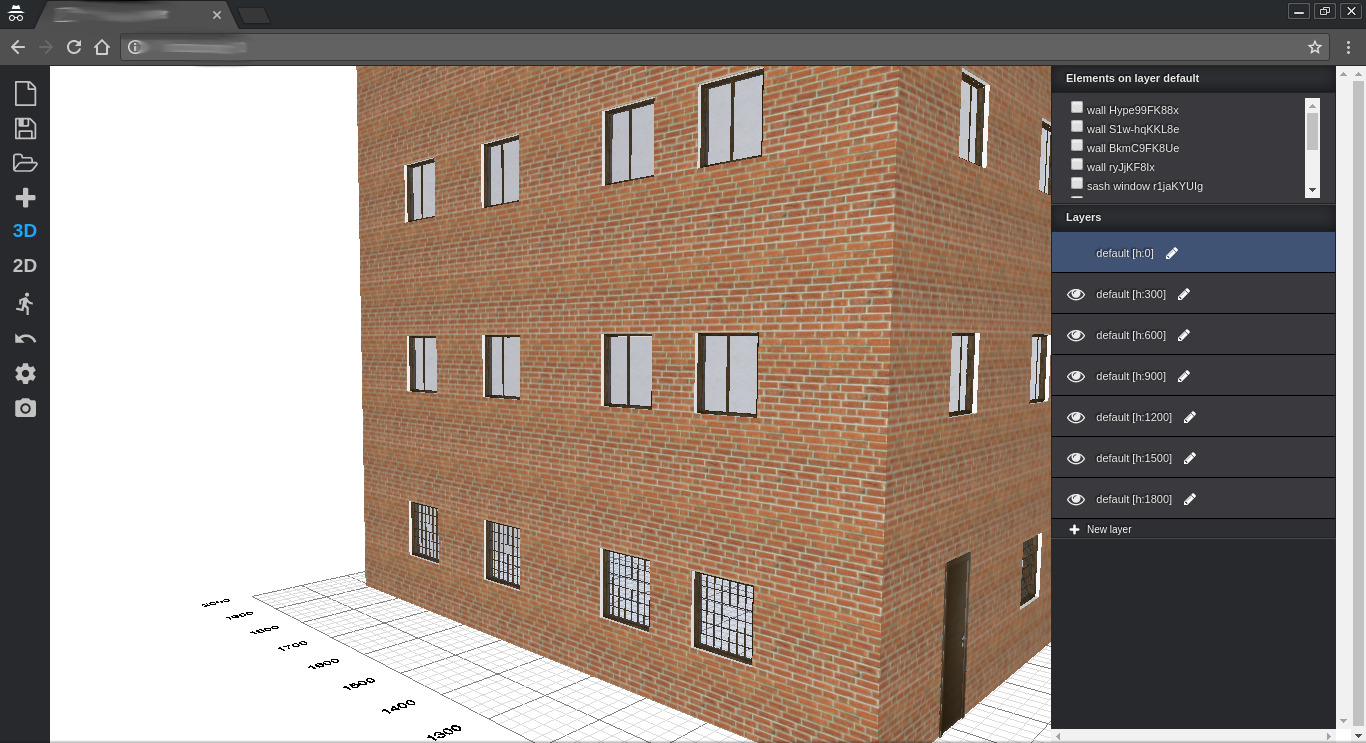
\includegraphics[width=\linewidth]{contents/images/palazzo2}
\caption{3D visualization of a building}
\label{fig3D-palace}
\end{figure}

Figures~\ref{fig3D-school} and~\ref{fig3D-palace} show some examples of 3D visualizations.

\section{Serverless Architecture}\label{sec:architecture}

We used a Serverless Architecture to deploy all the work.

To offer the application to end-users with high availability and high performance we deployed all Javascript files that are part of the system into a CDN (Content Delivery Network). This single point of deploy offered us a centralized method to upgrade all customers applications, whereby there is a new version, without any customer explicit action.

To perform CPU intensive operations, necessary to make complex geometric element, we used a third party FaaS system that run Python functions and that generate 3D elements. Thank to this we can scale up and down and adjust the CPU load on the traffic.

The application is distributed as frontend web application and so it's mostly executed into customer's browser. This has the following advantages: (i) to avoid user hard installation or updating typically performed by not technical users; (ii) to offer a good abstraction level that makes the application platform and operation system independent;  (iii) to avoid a server overloading by moving heavy computations on the user client.

The application state is mostly inside the customer's browser and it is represented as a tree structured object. This state can be serialized and saved on a BaaS system or downloaded as JSON file. The customer can restore the application state in any time using a preceding downloaded serialized version of the state. The system will adjust the user interface and the scene by means of the Virtual DOM and the diff and patch algorithm.

The collaboration part is based on a DBaaS, with the common state stored in an external DB provided by Firebase. Following this methodology we could also add user authentication features based on external BaaS providing all user management functionalities.

In Figure~\ref{fig_serverless} there is the architectural schema described above\\\\

\begin{figure}[htb]
\centering
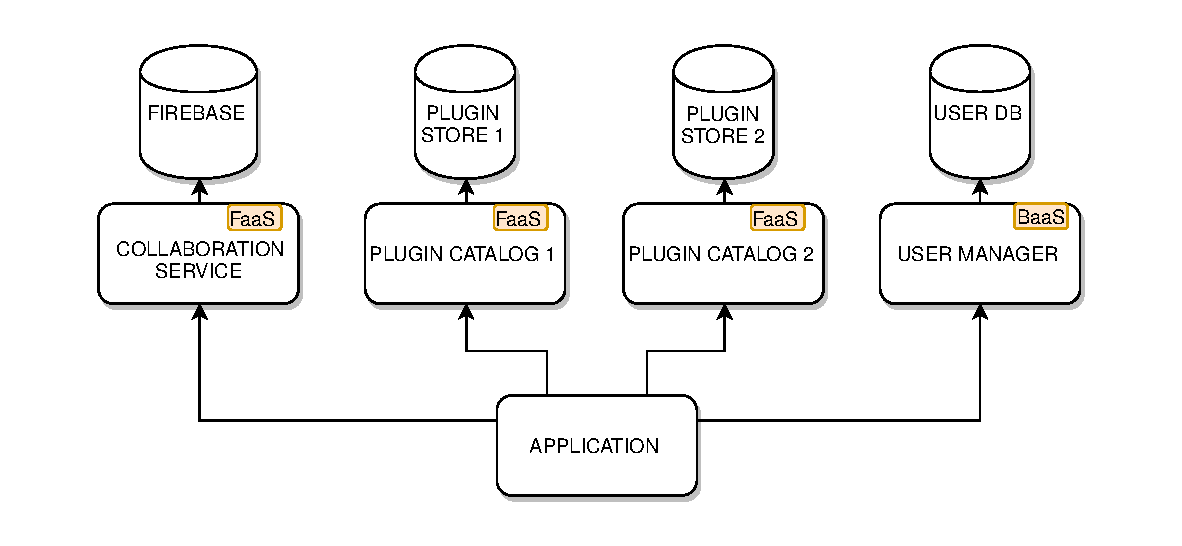
\includegraphics[width=\linewidth]{contents/images/serverless-diagram}

\caption{The serverless architecture for our application.}
\label{fig_serverless}
\end{figure}



\subsection{Centralized Application State}\label{ssub:centr_state}

blabla

\subsection{Component Based UI}


blabla
\section{Conclusions}\label{sec:conclusions}

In this work we outlined a serverless architecture to support buildings modeling in a Web environment. The serverless  architecture that gives benefits in terms of availability, reliability, scalability, easiness of deployment, maintainability and upgradability is obtained by implementing the application logic as a client-side only centralized state Web application exploiting the unidirectional data flow pattern. This approach allow for a easy-to-serialize state (in the form os a JSON document) that can be pushed on a third party document oriented DB-as-a-Service and loaded back in the frontend reactive architecture, which transparently reload the state once its serialized version is passed in. The application itself is served by a CDN (Content Delivery Network) thus avoiding any need for web server. Offline routines rely on Function-as-a-Service platform as well as users management and collaboration features.

This architecture has been successfully employed by the authors in the \emph{Metior} project~\cite{CITARE METIOR}, a tool to support selective deconstruction of buildings in the pursuit of a ``zero waste'' model.

%\section{Discussion \& Conclusion}\label{sec:conclusion}




% An example of a floating figure using the graphicx package.
% Note that \label must occur AFTER (or within) \caption.
% For figures, \caption should occur after the \includegraphics.
% Note that IEEEtran v1.7 and later has special internal code that
% is designed to preserve the operation of \label within \caption
% even when the captionsoff option is in effect. However, because
% of issues like this, it may be the safest practice to put all your
% \label just after \caption rather than within \caption{}.
%
% Reminder: the "draftcls" or "draftclsnofoot", not "draft", class
% option should be used if it is desired that the figures are to be
% displayed while in draft mode.
%
%\begin{figure}[!t]
%\centering
%\includegraphics[width=2.5in]{myfigure}
% where an .eps filename suffix will be assumed under latex, 
% and a .pdf suffix will be assumed for pdflatex; or what has been declared
% via \DeclareGraphicsExtensions.
%\caption{Simulation results for the network.}
%\label{fig_sim}
%\end{figure}

% Note that the IEEE typically puts floats only at the top, even when this
% results in a large percentage of a column being occupied by floats.


% An example of a double column floating figure using two subfigures.
% (The subfig.sty package must be loaded for this to work.)
% The subfigure \label commands are set within each subfloat command,
% and the \label for the overall figure must come after \caption.
% \hfil is used as a separator to get equal spacing.
% Watch out that the combined width of all the subfigures on a 
% line do not exceed the text width or a line break will occur.
%
%\begin{figure*}[!t]
%\centering
%\subfloat[Case I]{\includegraphics[width=2.5in]{box}%
%\label{fig_first_case}}
%\hfil
%\subfloat[Case II]{\includegraphics[width=2.5in]{box}%
%\label{fig_second_case}}
%\caption{Simulation results for the network.}
%\label{fig_sim}
%\end{figure*}
%
% Note that often IEEE papers with subfigures do not employ subfigure
% captions (using the optional argument to \subfloat[]), but instead will
% reference/describe all of them (a), (b), etc., within the main caption.
% Be aware that for subfig.sty to generate the (a), (b), etc., subfigure
% labels, the optional argument to \subfloat must be present. If a
% subcaption is not desired, just leave its contents blank,
% e.g., \subfloat[].


% An example of a floating table. Note that, for IEEE style tables, the
% \caption command should come BEFORE the table and, given that table
% captions serve much like titles, are usually capitalized except for words
% such as a, an, and, as, at, but, by, for, in, nor, of, on, or, the, to
% and up, which are usually not capitalized unless they are the first or
% last word of the caption. Table text will default to \footnotesize as
% the IEEE normally uses this smaller font for tables.
% The \label must come after \caption as always.
%
%\begin{table}[!t]
%% increase table row spacing, adjust to taste
%\renewcommand{\arraystretch}{1.3}
% if using array.sty, it might be a good idea to tweak the value of
% \extrarowheight as needed to properly center the text within the cells
%\caption{An Example of a Table}
%\label{table_example}
%\centering
%% Some packages, such as MDW tools, offer better commands for making tables
%% than the plain LaTeX2e tabular which is used here.
%\begin{tabular}{|c||c|}
%\hline
%One & Two\\
%\hline
%Three & Four\\
%\hline
%\end{tabular}
%\end{table}


% Note that the IEEE does not put floats in the very first column
% - or typically anywhere on the first page for that matter. Also,
% in-text middle ("here") positioning is typically not used, but it
% is allowed and encouraged for Computer Society conferences (but
% not Computer Society journals). Most IEEE journals/conferences use
% top floats exclusively. 
% Note that, LaTeX2e, unlike IEEE journals/conferences, places
% footnotes above bottom floats. This can be corrected via the
% \fnbelowfloat command of the stfloats package.







% conference papers do not normally have an appendix



% use section* for acknowledgment
\ifCLASSOPTIONcompsoc
  % The Computer Society usually uses the plural form
  \section*{Acknowledgments}

Authors would like to thank GEOWEB S.p.A., a web service company owned by Sogei S.p.A. and CNGeGL Italian National Board of Quantity Surveyors, for supporting this work. Thanks are extended to Stefano Perrone for developing the models shown in the Figures~\ref{FIGURE-CREATE-DA-STEFANO}.

\else
  % regular IEEE prefers the singular form
  \section*{Acknowledgment}
\fi



% trigger a \newpage just before the given reference
% number - used to balance the columns on the last page
% adjust value as needed - may need to be readjusted if
% the document is modified later
%\IEEEtriggeratref{8}
% The "triggered" command can be changed if desired:
%\IEEEtriggercmd{\enlargethispage{-5in}}

% references section

% can use a bibliography generated by BibTeX as a .bbl file
% BibTeX documentation can be easily obtained at:
% http://mirror.ctan.org/biblio/bibtex/contrib/doc/
% The IEEEtran BibTeX style support page is at:
% http://www.michaelshell.org/tex/ieeetran/bibtex/
\bibliographystyle{IEEEtran}
% argument is your BibTeX string definitions and bibliography database(s)
\bibliography{bare_conf_compsoc}
%
% <OR> manually copy in the resultant .bbl file
% set second argument of \begin to the number of references
% (used to reserve space for the reference number labels box)
% \begin{thebibliography}{1}
% 
% \bibitem{IEEEhowto:kopka}
% Esempio
% %H.~Kopka and P.~W. Daly, \emph{A Guide to \LaTeX}, 3rd~ed.\hskip 1em plus
% %  0.5em minus 0.4em\relax Harlow, England: Addison-Wesley, 1999.
% 
% \bibitem{IEEEhowto:kopka}
% https://tools.ietf.org/html/rfc6902
% 
% \end{thebibliography}




% that's all folks
\end{document}


